\section{Hierarchical Configuration Tuning}\label{sec:framework}

\subsection{Motivation and Tuning Objectives}

Configuration tuning in lossy compression usually involves multiple configuration dimensions rather than a single parameter. These dimensions may differ substantially in the size of their candidate spaces, their sensitivity to the input data, the cost of evaluating candidate choices, and the scope over which a selected configuration can be reused. Moreover, the choice made for one configuration dimension may affect the optimal choice for another, although the strength of such interactions varies across dimensions.

The objective of tuning is therefore not simply to identify the configuration with the best rate--distortion performance, but to obtain meaningful compression gains without introducing excessive tuning or execution overhead. Achieving this objective requires balancing the performance benefit of configuration exploration against the cost of evaluating and applying the resulting choices.

\subsection{Hierarchical Tuning Framework and Evaluation Strategies}

\begin{figure}[htb]
    \centering
    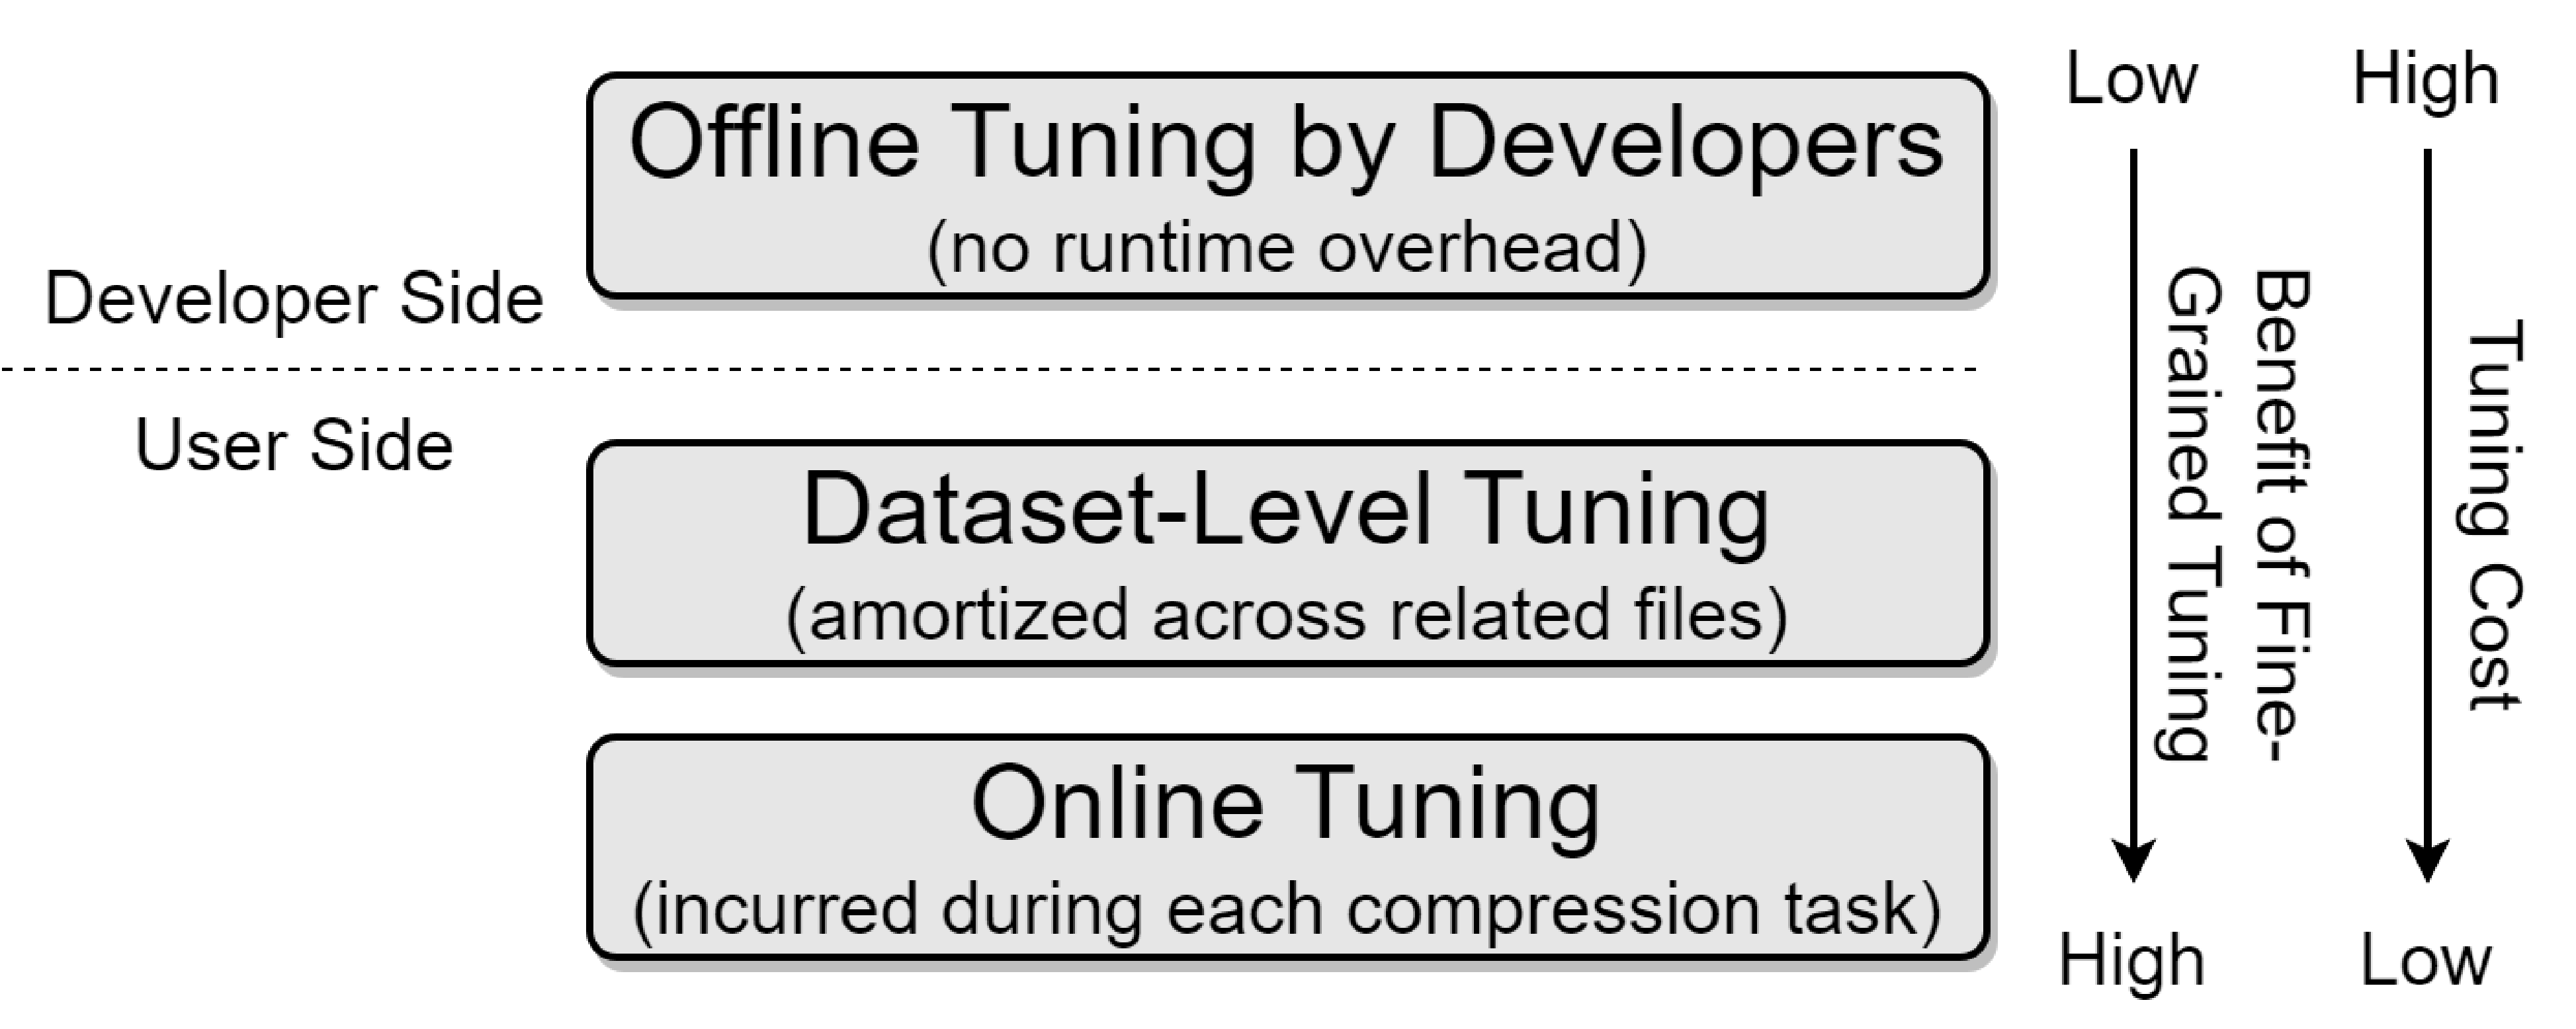
\includegraphics[width=0.7\linewidth]{figs/3/diagram1.pdf}
    \caption{Hierarchical Organization of Configuration Tuning}
    \label{fig:diagram1}
\end{figure}

Exploring all configuration dimensions uniformly at runtime is neither necessary nor practical. As illustrated in Figure~\ref{fig:diagram1}, we therefore assign different tuning steps to three stages: offline tuning performed by compressor developers across multiple datasets, dataset-level tuning performed before compression on representative data, and online tuning performed during compression for individual files or data blocks. Offline tuning introduces no runtime overhead for users, while dataset-level tuning costs can be amortized across related files. In contrast, online tuning costs are incurred during compression and must therefore remain sufficiently low.

The appropriate stage for each configuration dimension depends on its expected benefit and tuning cost. These two aspects are determined by several interrelated factors. We consider the following factors:

\begin{itemize}
\item \textbf{Regularity of the performance landscape} describes how smoothly and predictably compression performance changes as a numerical configuration varies while other configurations are fixed. If the response is smooth and approximately unimodal, a near-optimal value can often be identified using only a small number of evaluations. The regularity of the response may depend on the amount of data used for evaluation. Aggregating performance over an entire dataset or a large data region tends to average out local variations, whereas evaluation on a small data block may produce irregular fluctuations caused by its limited and highly localized data characteristics.

\item \textbf{Magnitude of the potential gain} describes the expected maximum performance improvement achievable through tuning relative to a fixed default choice. Dimensions with limited potential gains may not justify expensive or repeated tuning.

\item \textbf{Generalizability} describes whether a selected configuration can be reused across datasets or across related files, variables, or timesteps. Greater reuse allows the tuning overhead to be amortized over more compression tasks.

\item \textbf{Size of the candidate space} describes the number of possible choices and, consequently, the number of candidates that may need to be evaluated. For categorical or integer-valued configurations, the candidate space is explicitly defined. For continuous-valued configurations, however, its effective size depends on both the search range and the sampling resolution. The required resolution is further influenced by the regularity of the performance landscape and the magnitude of the potential tuning gain.

\item \textbf{Interaction with other configuration dimensions} describes the extent to which the best choice for one dimension depends on the choices made for other dimensions. Weakly interacting dimensions can be tuned independently or sequentially, while strongly interacting dimensions may require joint search.

\item \textbf{Availability and reliability of proxy metrics} describes whether candidate configurations can be evaluated without executing the complete compression pipeline. An inexpensive and sufficiently reliable proxy can enable fine-grained online tuning by reducing the per-candidate evaluation cost. However, a proxy that poorly preserves the relative ranking of candidates may lead to suboptimal decisions, even if it is inexpensive to compute.
\end{itemize}

These factors should be considered jointly rather than as independent assignment rules. Each factor indicates a tendency toward a particular tuning stage, so a configuration dimension may be suitable for more than one stage. The final assignment is therefore necessarily empirical and may involve trade-offs between data-specific adaptation and practical preprocessing and execution overhead.